\chapter{Números Naturais}
\section{Sistemas de numeração}
\begin{list}{\textbf{Questão \arabic{quest}.}}{\usecounter{quest}}
%define a margem da lista.	
%\setlength{\labelwidth}{-2mm} \setlength{\parsep}{0mm}
%\setlength{\topsep}{0mm} \setlength{\leftmargin}{-2mm}
\renewcommand{\labelenumi}{(\alph{enumi})}

\item Passe o número abaixo para o nosso sistema de numeração.
		\begin{multicols}{4}		
		\begin{enumerate}
			\item XX
			\item CM
			\item LXVII
			\item XLV
			\item XXXIX
			\item XIII
			\item MDCCLXXIX
			\item MCMLXIII
		\end{enumerate}
		\end{multicols}
		
		\item Escreva os números abaixo no sistema de numeração romano.
			\begin{multicols}{4}		
			\begin{enumerate}
				\item 18
				\item 352
				\item 29
				\item 734
				\item 97
				\item 3008
				\item 270
				\item 999
			\end{enumerate}
			\end{multicols}
			
		\item Passe do sistema de numeração romano para o nosso sistema.
		\begin{multicols}{3}		
		\begin{enumerate}
			\item $\overline{XXI}DCXL$
			\item $\overline{CLXX}$
			\item $\overline{\overline{CCC}}\ \overline{LXX}IV$
		\end{enumerate}
		\end{multicols}
		
		\item Qual o valor posicional no número 7 nos números abaixo?
		\begin{multicols}{3}		
		\begin{enumerate}
			\item 279
			\item 154 523 657
			\item 78 954
		\end{enumerate}
		\end{multicols}
		
		\item Escreva:			
		\begin{enumerate}
			\item Um número natural de cinco algarismo distintos no qual apareça o 2 no valor posicional 20;
			\item o menor número natural de quatro dígitos;
			\item o maior número natural de três algarismos distintos cuja a soma seja 6.
		\end{enumerate}
		
		\item O número 8 515 692 a ordem do algarismo 1 é a das dezenas de milhar e seu valor posicional é 10 000. Ainda em relação a esse número, responda.	
		\begin{enumerate}
			\item Qual é a ordem do algarismo 6? Qual o seu valor posicional?
			\item Qual é a ordem do algarismo 8? Qual o seu valor posicional?
			\item Quantas classe tem esse número?
			\item Quantas ordens tem esse número?
		\end{enumerate}
		
		\item Escreva como se leem o número abaixo.
		\begin{multicols}{4}		
		\begin{enumerate}
			\item 5 136 784
			\item 6 002 457
			\item 9 000 020
			\item 787 000 874 125
		\end{enumerate}
		\end{multicols}
		
		\item Escreva o número formado por:
		\begin{enumerate}
				\item seis dezenas de milhão, mais três centenas de milhar, mais nove dezenas.
				\item três unidades de milhão, mais cinco unidades de milhar, mais duas unidades.
		\end{enumerate}
		
		\item Represente com todos os algarismos.
		\begin{multicols}{3}		
		\begin{enumerate}
			\item 4,8 mil
			\item 3,6 milhões
			\item 2,7 bilhões.
		\end{enumerate}
		\end{multicols}
		
		\item Escreva na forma simplificada, com palavras e algarismo.
		\begin{multicols}{2}		
		\begin{enumerate}
			\item 10 400 000
			\item 13 500
			\item 2 000 500 000
			\item 8 000 000 000 000 
		\end{enumerate}
		\end{multicols}
		
		\item Escreva na forma simplificada (usando vírgula).
		\begin{multicols}{4}		
		\begin{enumerate}
			\item 9 600 000
			\item 23 500
			\item 8 600
			\item 6 600
		\end{enumerate}
		\end{multicols}
		
		\item Identifique qual ideia da adição está envolvida em cada situação e responda às questões.
		\begin{enumerate}
			\item Marcelo tinha 123 reais e ganhou de sua tia uma nota de 50 reais. Com quanto ele ficou?
			\item A coleção de Marta tem 60 adesivos e a de Aninha tem 50 adesivos. Reunindo as duas coleções, quantos adesivos elas têm?
			\item De 1º de junho a 31 de julho do mesmo ano, incluindo esses dias, quantos dias temos?
			\item Pedro já caminhou 1450 metros. Se caminhar outros 500 metros, vai completar um percurso de quantos metros?
		\end{enumerate}
		
		\item Elabore um problema que envolva uma adição.
		
		\item Use o algoritmo da decomposição para resolver a situação a seguir: Jonas tinha 624 reais na poupança e depositou 142 reais. Quanto ele tem agora de saldo na poupança?
		\item Explique com suas palavras por que o zero é chamando de elemento neutro da adição.
		
		\item No início do mês, no estoque de uma loja de brinquedos havia 2174 bonecos articulados. Durante a semana, foram vendidos 1268 bonecos. Quantos bonecos restaram?
		
		\item Efetue estas subtrações usando o algoritmo da  decomposição do subtraendo.		
		\begin{multicols}{4}
		\begin{enumerate}
			\item $497-54$
			\item $1239-129$
			\item $795-148$
			\item $2914-1825$
		\end{enumerate}
		\end{multicols}
		
		\item Um \textit{pet shop} teve, no mês de março, uma despesa de 4256 reais e um faturamento de 7250 reais. Nesse mês houve lucro ou prejuízo? De quanto?
		\item Pedro tinha 567 selos. Deu 45 para Carla, 39 para Beto e 27 para Bia. Com quantos selos ele ficou?
		\item Descubra os algarismos que faltam em cada um dos algoritmos abaixo:
		\begin{multicols}{2}
		\begin{enumerate}
			\item 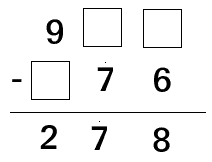
\includegraphics[scale=0.4]{figuras/fig66.png}
			\item 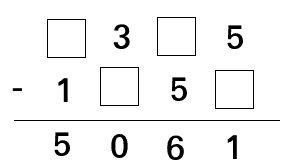
\includegraphics[scale=0.4]{figuras/fig67.png}
		\end{enumerate}
		\end{multicols}
		
\end{list}